\documentclass[]{beamer}\usepackage[]{graphicx}\usepackage[]{color}
% maxwidth is the original width if it is less than linewidth
% otherwise use linewidth (to make sure the graphics do not exceed the margin)
\makeatletter
\def\maxwidth{ %
  \ifdim\Gin@nat@width>\linewidth
    \linewidth
  \else
    \Gin@nat@width
  \fi
}
\makeatother

\definecolor{fgcolor}{rgb}{0.345, 0.345, 0.345}
\newcommand{\hlnum}[1]{\textcolor[rgb]{0.686,0.059,0.569}{#1}}%
\newcommand{\hlstr}[1]{\textcolor[rgb]{0.192,0.494,0.8}{#1}}%
\newcommand{\hlcom}[1]{\textcolor[rgb]{0.678,0.584,0.686}{\textit{#1}}}%
\newcommand{\hlopt}[1]{\textcolor[rgb]{0,0,0}{#1}}%
\newcommand{\hlstd}[1]{\textcolor[rgb]{0.345,0.345,0.345}{#1}}%
\newcommand{\hlkwa}[1]{\textcolor[rgb]{0.161,0.373,0.58}{\textbf{#1}}}%
\newcommand{\hlkwb}[1]{\textcolor[rgb]{0.69,0.353,0.396}{#1}}%
\newcommand{\hlkwc}[1]{\textcolor[rgb]{0.333,0.667,0.333}{#1}}%
\newcommand{\hlkwd}[1]{\textcolor[rgb]{0.737,0.353,0.396}{\textbf{#1}}}%
\let\hlipl\hlkwb

\usepackage{framed}
\makeatletter
\newenvironment{kframe}{%
 \def\at@end@of@kframe{}%
 \ifinner\ifhmode%
  \def\at@end@of@kframe{\end{minipage}}%
  \begin{minipage}{\columnwidth}%
 \fi\fi%
 \def\FrameCommand##1{\hskip\@totalleftmargin \hskip-\fboxsep
 \colorbox{shadecolor}{##1}\hskip-\fboxsep
     % There is no \\@totalrightmargin, so:
     \hskip-\linewidth \hskip-\@totalleftmargin \hskip\columnwidth}%
 \MakeFramed {\advance\hsize-\width
   \@totalleftmargin\z@ \linewidth\hsize
   \@setminipage}}%
 {\par\unskip\endMakeFramed%
 \at@end@of@kframe}
\makeatother

\definecolor{shadecolor}{rgb}{.97, .97, .97}
\definecolor{messagecolor}{rgb}{0, 0, 0}
\definecolor{warningcolor}{rgb}{1, 0, 1}
\definecolor{errorcolor}{rgb}{1, 0, 0}
\newenvironment{knitrout}{}{} % an empty environment to be redefined in TeX

\usepackage{alltt}
%\documentclass[handout]{beamer}
% ***************************************************************
% for handout, change only this...
%   \documentclass[twocolumn]{article}
%   \usepackage{beamerarticle}
%   \setlength{\textwidth}{7.5in}
%   \setlength{\textheight}{9.8in}
%   \setlength{\topmargin}{-1in}
%   \setlength{\oddsidemargin}{-.52in}
%   \setlength{\evensidemargin}{-.52in}

%\usepackage{beamerprosper}
%\usetheme{Warsaw}
%\usecolortheme{orchid}

\usepackage{graphicx}
\usepackage{amsmath,amssymb,array,comment,eucal}
\usepackage{xcolor}
\definecolor{beamer@blendedblue}{RGB}{86,155,189}
\definecolor{myblue}{RGB}{12,76,138}
\setbeamercolor{structure}{fg=myblue}
\definecolor{Ftitle}{RGB}{12,76,138}
\definecolor{Descitem}{RGB}{238,238,244}
\definecolor{StdTitle}{RGB}{12,76,138}
\definecolor{StdBody}{RGB}{213,24,0}
\definecolor{StdBody}{RGB}{213,24,0}

\definecolor{AlTitle}{RGB}{255, 190, 190}
\definecolor{AlBody}{RGB}{213,24,0}

\definecolor{ExTitle}{RGB}{201, 217, 217}
\definecolor{ExBody}{RGB}{213,24,0}

\setbeamercolor{frametitle}{fg = Ftitle}
\setbeamercolor{title}{fg = Ftitle}
\setbeamercolor{item}{fg = Ftitle}
\setbeamercolor{subitem}{fg = Ftitle}
\setbeamercolor{subsubitem}{fg = Ftitle}
\setbeamercolor{description item}{fg = myblue}
\setbeamercolor{titlelike}{fg=myblue}

\DeclareMathOperator{\sgn}{sgn}
\newcommand{\e}{\mathbf{e}}
\renewcommand{\P}{\mathbf{P}}
\newcommand{\F}{\mathbf{F}}
\newcommand{\R}{\textsf{R}}
\newcommand{\mat}[1] {\mathbf{#1}}
%\newcommand{\ind}{\mathrel{\mathop{\sim}\limits^{\mathit{ind}}}}
%\newcommand{\iid}{\mathrel{\mathop{\sim}\limits^{\mathit{iid}}}}
\newcommand{\E}{\textsf{E}}
\newcommand{\SE}{\textsf{SE}}
\newcommand{\SSE}{\textsf{SSE}}
\newcommand{\RSS}{\textsf{RSS}}
\newcommand{\FSS}{\textsf{FSS}}
\renewcommand{\SS}{\textsf{SS}}
\newcommand{\MSE}{\textsf{MSE}}
\newcommand{\SSR}{\textsf{SSR}}
\newcommand{\Be}{\textsf{Beta}}
\newcommand{\St}{\textsf{St}}
\newcommand{\Ca}{\textsf{C}}
\newcommand{\Exp}{\textsf{Exp}}
\newcommand{\GDP}{\textsf{GDP}}
\newcommand{\NcSt}{\textsf{NcSt}}
\newcommand{\Bin}{\textsf{Bin}}
\newcommand{\NB}{\textsf{NegBin}}
\renewcommand{\NG}{\textsf{NG}}
\newcommand{\N}{\textsf{N}}
\newcommand{\Ber}{\textsf{Ber}}
\newcommand{\Poi}{\text{Poi}}
\newcommand{\Gam}{\textsf{Gamma}}
\newcommand{\BB}{\textsf{BB}}
\newcommand{\Gm}{\textsf{G}}
\newcommand{\Un}{\textsf{Unif}}
\newcommand{\Ex}{\textsf{Exp}}
\newcommand{\DE}{\textsf{DE}}
\newcommand{\tr}{\textsf{tr}}
\newcommand{\cF}{{\cal{F}}}
\newcommand{\cL}{{\cal{L}}}
\newcommand{\cI}{{\cal{I}}}
\newcommand{\cB}{{\cal{B}}}
\newcommand{\cP}{{\cal{P}}}
\newcommand{\bbR}{\mathbb{R}}
\newcommand{\bbN}{\mathbb{N}}
\newcommand{\pperp}{\mathrel{{\rlap{$\,\perp$}\perp\,\,}}}
\newcommand{\OFP}{(\Omega,\cF, \P)}
\newcommand{\eps}{\boldsymbol{\epsilon}}
\newcommand{\1}{\mathbf{1}_n}
\newcommand{\gap}{\vspace{8mm}}
\newcommand{\ind}{\mathrel{\mathop{\sim}\limits^{\rm ind}}}
\newcommand{\simiid}{\ensuremath{\mathrel{\mathop{\sim}\limits^{\rm
iid}}}}
\newcommand{\eqindis}{\ensuremath{\mathrel{\mathop{=}\limits^{\rm D}}}}
\newcommand{\iid}{\textit{i.i.d.}}
\newcommand{\SSZ}{S_{zz}}
\newcommand{\SZW}{S_{zw}}
\newcommand{\Var}{\textsf{Var}}
\newcommand{\corr}{\textsf{corr}}
\newcommand{\diag}{\textsf{diag}}
\newcommand{\var}{\textsf{var}}
\newcommand{\Cov}{\textsf{Cov}}
\newcommand{\Sam}{{\cal S}}
\def\H{\mathbf{H}}
\newcommand{\I}{\mathbf{I}}
\newcommand{\Y}{\mathbf{Y}}
\newcommand{\tY}{\tilde{\mathbf{Y}}}
\newcommand{\Yhat}{\hat{\mathbf{Y}}}
\newcommand{\Yobs}{\mathbf{Y}_{{\cal S}}}
\newcommand{\barYobs}{\bar{Y}_{{\cal S}}}
\newcommand{\barYmiss}{\bar{Y}_{{\cal S}^c}}
\def\bv{\mathbf{b}}
\def\X{\mathbf{X}}
\def\tX{\tilde{\mathbf{X}}}
\def\x{\mathbf{x}}
\def\xbar{\bar{\mathbf{x}}}
\def\Xbar{\bar{\mathbf{X}}}
\def\Xg{\mathbf{X}_{\boldsymbol{\gamma}}}
\def\Ybar{\bar{\Y}}
\def\ybar{\bar{y}}
\def\y{\mathbf{y}}
\def\Yf{\mathbf{Y_f}}
\def\W{\mathbf{W}}
\def\L{\mathbf{L}}
\def\w{\mathbf{w}}
\def\U{\mathbf{U}}
\def\V{\mathbf{V}}
\def\Q{\mathbf{Q}}
\def\Z{\mathbf{Z}}
\def\z{\mathbf{z}}
\def\v{\mathbf{v}}
\def\u{\mathbf{u}}

\def\zero{\mathbf{0}}
\newcommand{\one}{\mathbf{1}}
\newcommand{\taub}{\boldsymbol{\tau}}
\newcommand{\betav}{\boldsymbol{\beta}}
\newcommand{\alphav}{\boldsymbol{\alpha}}
\newcommand{\A}{\mathbf{A}}
\def\a{\mathbf{a}}
\def\K{\mathbf{K}}
\newcommand{\B}{\mathbf{B}}
\def\b{\boldsymbol{\beta}}
\def\bhat{\hat{\boldsymbol{\beta}}}
\def\btilde{\tilde{\boldsymbol{\beta}}}
\def\tb{\boldsymbol{\theta}}
\def\bg{\boldsymbol{\beta_\gamma}}
\def\bgnot{\boldsymbol{\beta_{(-\gamma)}}}
\def\mub{\boldsymbol{\mu}}
\def\tmub{\tilde{\boldsymbol{\mu}}}
\def\muhat{\hat{\boldsymbol{\mu}}}
\def\tb{\boldsymbol{\theta}}
\def\tk{\boldsymbol{\theta}_k}
\def\tj{\boldsymbol{\theta}_j}
\def\Mk{\boldsymbol{{\cal M}}_k}
\def\M{\boldsymbol{{\cal M}}}
\def\Mj{\boldsymbol{{\cal M}}_j}
\def\Mi{\boldsymbol{{\cal M}}_i}
\def\Mg{{\boldsymbol{{\cal M}_\gamma}}}
\def\Mnull{\boldsymbol{{\cal M}}_{N}}
\def\gMPM{\boldsymbol{\gamma}_{\text{MPM}}}
\def\gHPM{\boldsymbol{\gamma}_{\text{HPM}}}
\def\Mfull{\boldsymbol{{\cal M}}_{F}}
\def\tg{\boldsymbol{\theta}_{\boldsymbol{\gamma}}}
\def\g{\boldsymbol{\gamma}}
\def\eg{\boldsymbol{\eta}_{\boldsymbol{\gamma}}}
\def\G{\mathbf{G}}
\def\cM{\cal M}
\def\D{\Delta}
\def \shat{{\hat{\sigma}}^2}
\def\uv{\mathbf{u}}
\def\l {\lambda}
\def\d{\delta}
\def\Sigmab{\boldsymbol{\Sigma}}
\def\Lambdab{\boldsymbol{\Lambda}}
\def\lambdab{\boldsymbol{\lambda}}
\def\Mg{{\cal M}_\gamma}
\def\S{{\cal{S}}}
\def\qg{p_{\boldsymbol{\gamma}}}
\def\pg{p_{\boldsymbol{\gamma}}}
%\def\t{\mathbf{t}}
\def\T{\boldsymbol{\Theta}}
\def\Tb{\boldsymbol{\Theta}}

\title{BMA \&  Distributions }
 
\author{Hoff Chapter 9, Liang et al 2008, Hoeting et al (1999), Clyde \&
 George (2004)}
\date{\today}
%\Logo(-1.9,7.3){
\includegraphics[width=.5in]{../eps/duke}}
% Optional: text to put in the bottom of each slide.
% By default, the title of the talk will be placed there.
%\slideCaption{\textit{October 28, 2005 }}
\IfFileExists{upquote.sty}{\usepackage{upquote}}{}
\begin{document}
%\SweaveOpts{concordance=TRUE}
% make the title slide
\maketitle




\begin{frame}[fragile]
\frametitle{USair Data}
\begin{knitrout}
\definecolor{shadecolor}{rgb}{0.969, 0.969, 0.969}\color{fgcolor}\begin{kframe}
\begin{alltt}
\hlkwd{library}\hlstd{(BAS)}
\hlkwd{data}\hlstd{(usair,} \hlkwc{package}\hlstd{=}\hlstr{"HH"}\hlstd{)}
\hlstd{poll.bma} \hlkwb{=} \hlkwd{bas.lm}\hlstd{(}\hlkwd{log}\hlstd{(SO2)} \hlopt{~} \hlstd{temp} \hlopt{+} \hlkwd{log}\hlstd{(mfgfirms)} \hlopt{+}
                             \hlkwd{log}\hlstd{(popn)} \hlopt{+} \hlstd{wind} \hlopt{+}
                             \hlstd{precip} \hlopt{+} \hlstd{raindays,}
                  \hlkwc{data}\hlstd{=usair,}
                  \hlkwc{prior}\hlstd{=}\hlstr{"g-prior"}\hlstd{,}
                  \hlkwc{alpha}\hlstd{=}\hlkwd{nrow}\hlstd{(usair),} \hlcom{# g = n}
                  \hlkwc{n.models}\hlstd{=}\hlnum{2}\hlopt{^}\hlnum{6}\hlstd{,}
                  \hlkwc{modelprior} \hlstd{=} \hlkwd{uniform}\hlstd{(),}
                  \hlkwc{method}\hlstd{=}\hlstr{"deterministic"}\hlstd{)}
\end{alltt}
\end{kframe}
\end{knitrout}

% Marginal Posterior Inclusion Probabilities:
% Intercept  temp   log(mfgfirms)  log(popn)   wind  precip  raindays
%   1.0000   0.9755       0.7190     0.2757  0.7654  0.5994   0.3104

\end{frame}

\begin{frame}[fragile]\frametitle{Summary}

\begin{small}
\begin{knitrout}
\definecolor{shadecolor}{rgb}{0.969, 0.969, 0.969}\color{fgcolor}\begin{kframe}
\begin{alltt}
\hlkwd{summary}\hlstd{(poll.bma)}
\end{alltt}
\begin{verbatim}
##               P(B != 0 | Y)  model 1   model 2   model 3   model 4   model 5
## Intercept         1.0000000 1.000000 1.0000000 1.0000000 1.0000000 1.0000000
## temp              0.9755041 1.000000 1.0000000 1.0000000 1.0000000 1.0000000
## log(mfgfirms)     0.7190313 1.000000 1.0000000 1.0000000 1.0000000 0.0000000
## log(popn)         0.2756811 0.000000 0.0000000 0.0000000 1.0000000 1.0000000
## wind              0.7654485 1.000000 1.0000000 1.0000000 1.0000000 1.0000000
## precip            0.5993801 1.000000 0.0000000 0.0000000 1.0000000 1.0000000
## raindays          0.3103574 0.000000 1.0000000 0.0000000 0.0000000 0.0000000
## BF                       NA 1.000000 0.3022674 0.2349056 0.2093987 0.1971979
## PostProbs                NA 0.275800 0.0834000 0.0648000 0.0577000 0.0544000
## R2                       NA 0.542700 0.5130000 0.4558000 0.5500000 0.5020000
## dim                      NA 5.000000 5.0000000 4.0000000 6.0000000 5.0000000
## logmarg                  NA 7.616228 6.4197847 6.1676565 6.0527128 5.9926805
\end{verbatim}
\end{kframe}
\end{knitrout}
\end{small}

\end{frame}
\begin{frame}[fragile]\frametitle{Plots}

\centering
\begin{knitrout}
\definecolor{shadecolor}{rgb}{0.969, 0.969, 0.969}\color{fgcolor}\begin{kframe}
\begin{alltt}
 \hlstd{beta} \hlkwb{=} \hlkwd{coef}\hlstd{(poll.bma)}
 \hlkwd{par}\hlstd{(}\hlkwc{mfrow}\hlstd{=}\hlkwd{c}\hlstd{(}\hlnum{2}\hlstd{,}\hlnum{3}\hlstd{));}  \hlkwd{plot}\hlstd{(beta,} \hlkwc{subset}\hlstd{=}\hlnum{2}\hlopt{:}\hlnum{7}\hlstd{,}\hlkwc{ask}\hlstd{=F)}
\end{alltt}
\end{kframe}
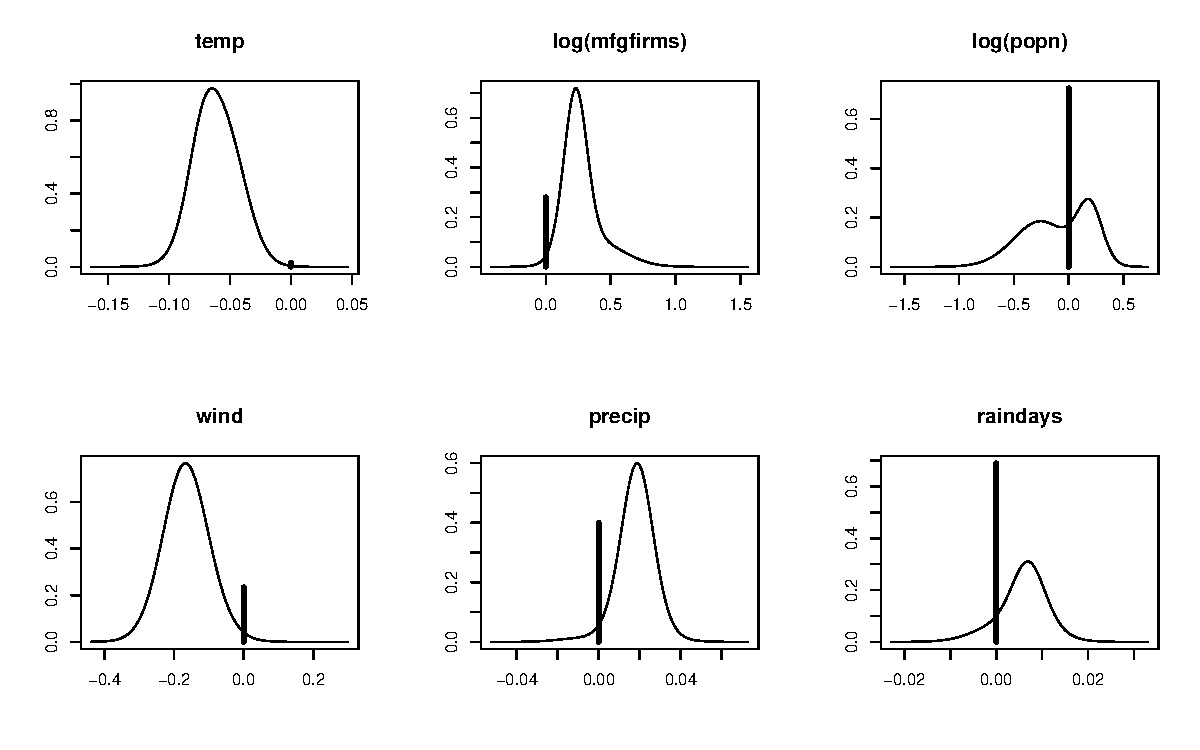
\includegraphics[width=0.75\linewidth,height=0.75\textheight]{figure/coef_plot-1} 
\end{knitrout}
\end{frame}

\begin{frame}\frametitle{Posterior Distribution  with Uniform Prior on Model Space}


\begin{knitrout}
\definecolor{shadecolor}{rgb}{0.969, 0.969, 0.969}\color{fgcolor}\begin{kframe}
\begin{alltt}
\hlkwd{image}\hlstd{(poll.bma,} \hlkwc{rotate}\hlstd{=}\hlnum{FALSE}\hlstd{)}
\end{alltt}
\end{kframe}
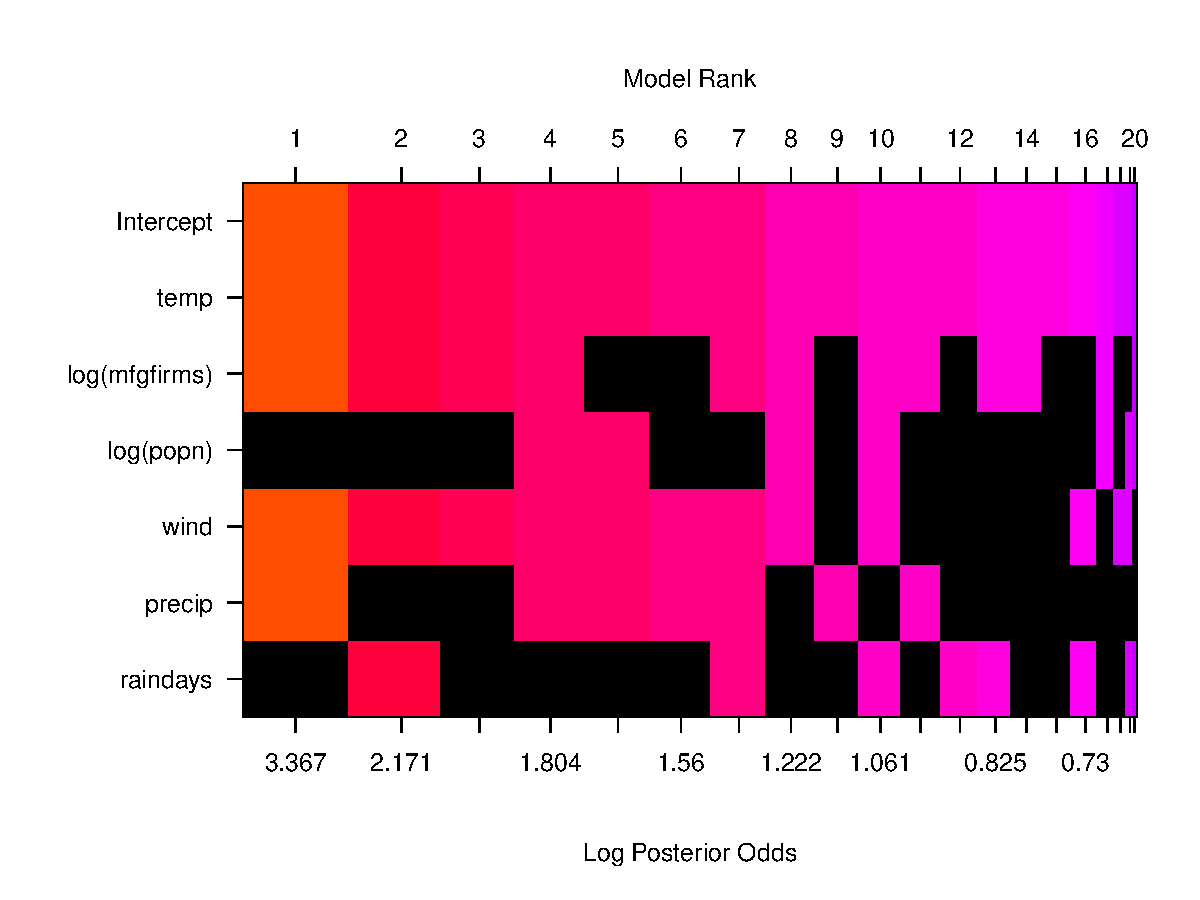
\includegraphics[width=4.5in,height=3in]{figure/unnamed-chunk-3-1} 
\end{knitrout}


\end{frame}

\begin{frame}[fragile]\frametitle{Posterior Distribution  with BB(1,1) Prior on Model Space}


\begin{knitrout}
\definecolor{shadecolor}{rgb}{0.969, 0.969, 0.969}\color{fgcolor}\begin{kframe}
\begin{alltt}
\hlstd{poll.bb.bma} \hlkwb{=} \hlkwd{bas.lm}\hlstd{(}\hlkwd{log}\hlstd{(SO2)} \hlopt{~} \hlstd{temp} \hlopt{+} \hlkwd{log}\hlstd{(mfgfirms)} \hlopt{+}
                                \hlkwd{log}\hlstd{(popn)} \hlopt{+} \hlstd{wind} \hlopt{+}
                                \hlstd{precip} \hlopt{+} \hlstd{raindays,}
                     \hlkwc{data}\hlstd{=usair,}
                     \hlkwc{prior}\hlstd{=}\hlstr{"g-prior"}\hlstd{,}
                     \hlkwc{alpha}\hlstd{=}\hlkwd{nrow}\hlstd{(usair),}
                     \hlkwc{n.models}\hlstd{=}\hlnum{2}\hlopt{^}\hlnum{6}\hlstd{,}  \hlcom{#enumerate}
                     \hlkwc{modelprior}\hlstd{=}\hlkwd{beta.binomial}\hlstd{(}\hlnum{1}\hlstd{,}\hlnum{1}\hlstd{))}
\end{alltt}
\end{kframe}
\end{knitrout}

\end{frame}

\begin{frame}\frametitle{BB(1,1) Prior on Model Space}


\begin{knitrout}
\definecolor{shadecolor}{rgb}{0.969, 0.969, 0.969}\color{fgcolor}\begin{kframe}
\begin{alltt}
\hlkwd{image}\hlstd{(poll.bb.bma,} \hlkwc{rotate}\hlstd{=}\hlnum{FALSE}\hlstd{)}
\end{alltt}
\end{kframe}
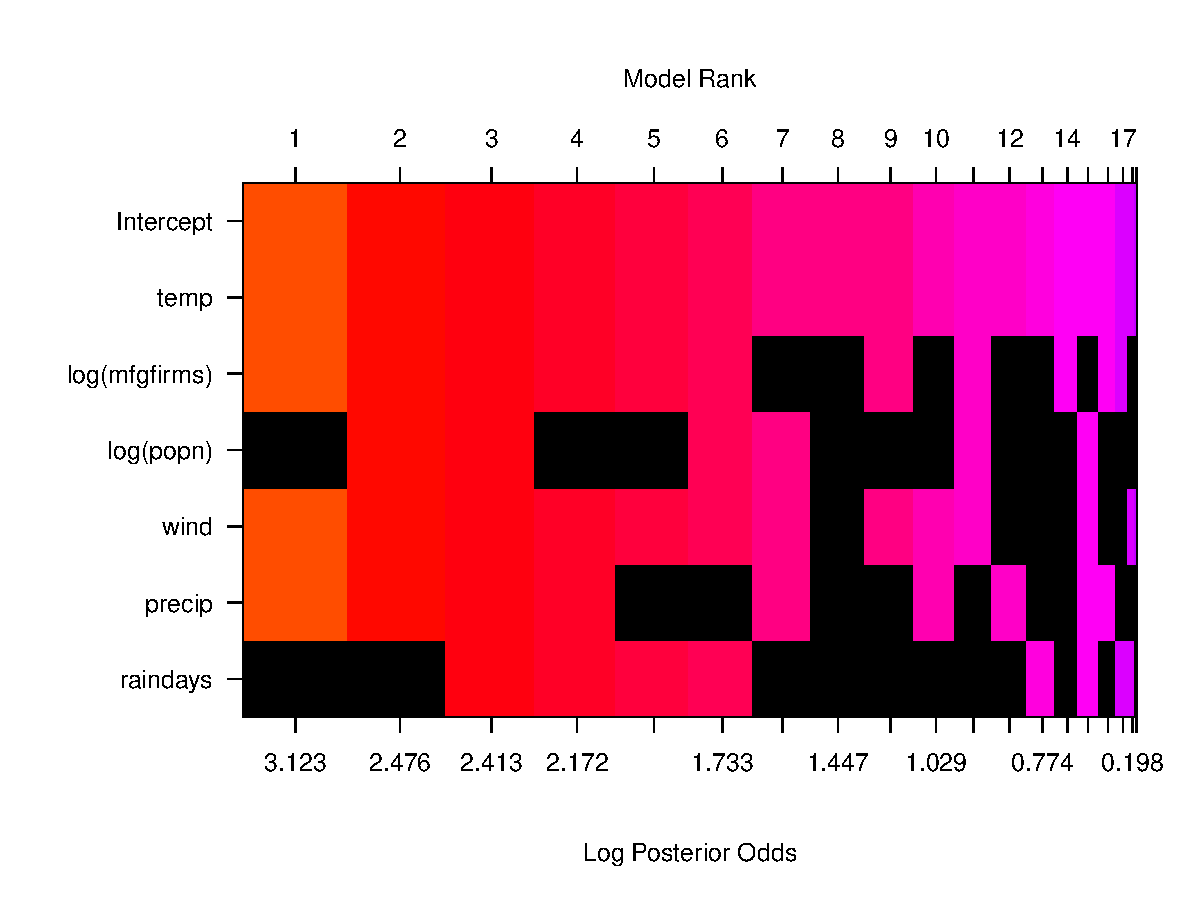
\includegraphics[width=4.5in,height=3in]{figure/unnamed-chunk-5-1} 
\end{knitrout}
\end{frame}


\begin{frame} \frametitle{Bartlett's Paradox}


The Bayes factor for comparing $\g$ to the null
model:
$$
 BF(\g : \g0) =    (1 + g)^{(n - 1 - \pg)/2} (1 + g(1 - R_{\g}^2))^{-(n-1)/2}
$$
\pause
\begin{itemize}
\item For fixed sample size $n$ and $R_{\g}^2$, consider taking values of  $g$ that
  go to infinity  \pause
\item Increasing vagueness in prior \pause
\item What happens to BF as $g \to \infty$? \pause
\item why is this a paradox?

\end{itemize}
\end{frame}



\begin{frame}
  \frametitle{Information Paradox}

The Bayes factor for comparing $\g$ to the null
model:
$$
 BF(\g : \g_0) =    (1 + g)^{(n - 1 - \pg)/2} (1 + g(1 - R_{\g}^2))^{-(n-1)/2}
$$
\pause
\begin{itemize}
\item Let $g$ be a fixed constant and take $n$ fixed. \pause
\item Let $F = \frac{R_{\g}^2/\pg}{(1 - R_{\g}^2)/(n - 1 - \pg)}$ \pause
\item As $R^2_{\g} \to 1$, $F \to \infty$ LR test would reject $\g_0$
  where $F$ is the usual $F$ statistic for  comparing model $\g$ to
  $\g_0$ \pause
\item BF converges to a fixed constant $(1+g)^{n - 1 -\pg/2}$  (does not go
  to infinity 
\end{itemize}

``Information Inconsistency''  see Liang et al JASA 2008


\end{frame}


\begin{frame}
  \frametitle{Mixtures of $g$ priors \& Information consistency}


\begin{itemize}
\item Need $BF \to \infty$ if $\R_{\g}^2 \to 1$
\item Put a prior on $g$
$$BF(\g : \g_0) =  \frac{ C \int (1 + g)^{(n - 1 - \pg)/2} (1 + g(1 - R_{\g}^2))^{-(n-1)/2} \pi(g) dg}{C}$$
\item interchange limit and integration as $R^2 \to 1$
want
$$ \E_g[(1 +
g)^{(n-1-\pg)/2}]$$  to diverge

\item hyper-g prior (Liang et al JASA 2008)
$$p(g) = \frac{a-2}{2}(1 + g)^{-a/2}$$ or $g/(1+g) \sim Beta(1, (a-2)/2)$

\item prior expectation converges if $a > n + 1 - \pg$

\item Consider minimal model $\pg = 1$ and $n = 3$ (can estimate intercept, one coefficient, and  $\sigma^2$, then $a > 3$ integral exists

\item For $2 < a \le 3$ integral diverges and resolves the information paradox!
\end{itemize}

\end{frame}

\begin{frame}
  \frametitle{Mixtures of $g$ priors \& Information consistency}

Need $BF \to \infty$ if $\R^2 \to 1$  $\Leftrightarrow$ $\E_g[(1 +
g)^{(n-1-\pg)/2}]$ diverges  (proof in Liang et al)
\pause
\begin{itemize}

\item hyper-g prior (Liang et al JASA 2008)
$$p(g) = \frac{a-2}{2}(1 + g)^{-a/2}$$ or $g/(1+g) \sim Beta(1, (a-2)/2)$
need $2 < a \le 3$
\pause
\item Jeffreys prior on $g$ corresponds to $a = 2$ (improper) \pause
\item Hyper-g/n  $(g/n)(1 + g/n) \sim (Beta(1, (a-2)/2)$ \pause
\item Zellner-Siow Cauchy prior $1/g \sim G(1/2, n/2)$ \pause
\item robust prior (Bayarri et al Annals of Statistics 2012 \pause
\item Intrinsic prior (Womack et al  JASA 2015)
\end{itemize}

 All have prior tails for $\b$  that behave like a Cauchy distribution
 and (the latter 4) marginal  likelihoods that can be computed using special hypergeometric
 functions   ($_2F_1$, Appell $F_1$)
\end{frame}



\begin{frame}\frametitle{Computation}

If $p > 35$  enumeration is difficult

  \begin{itemize}
  \item Gibbs sampler or Random-Walk algorithm on $\g$ \pause
  \item slow convergence/poor mixing with high correlations \pause
  \item Metropolis Hastings algorithms more flexibility \pause
        (swap pairs of variables)

\end{itemize}

\end{frame}


\begin{frame}[fragile] \frametitle{Diabetes Example from Hoff $p=64$ }

\begin{knitrout}
\definecolor{shadecolor}{rgb}{0.969, 0.969, 0.969}\color{fgcolor}\begin{kframe}
\begin{alltt}
\hlkwd{set.seed}\hlstd{(}\hlnum{8675309}\hlstd{)}
\hlkwd{source}\hlstd{(}\hlstr{"yX.diabetes.train.txt"}\hlstd{)}
\hlstd{diabetes.train} \hlkwb{=} \hlkwd{as.data.frame}\hlstd{(diabetes.train)}

\hlkwd{source}\hlstd{(}\hlstr{"yX.diabetes.test.txt"}\hlstd{)}
\hlstd{diabetes.test} \hlkwb{=} \hlkwd{as.data.frame}\hlstd{(diabetes.test)}
\hlkwd{colnames}\hlstd{(diabetes.test)[}\hlnum{1}\hlstd{]} \hlkwb{=} \hlstr{"y"}

\hlkwd{str}\hlstd{(diabetes.train)}
\end{alltt}
\begin{verbatim}
## 'data.frame':	342 obs. of  65 variables:
##  $ y      : num  -0.0147 -1.0005 -0.1444 0.6987 -0.2222 ...
##  $ age    : num  0.7996 -0.0395 1.7913 -1.8703 0.113 ...
##  $ sex    : num  1.064 -0.937 1.064 -0.937 -0.937 ...
##  $ bmi    : num  1.296 -1.081 0.933 -0.243 -0.764 ...
##  $ map    : num  0.459 -0.553 -0.119 -0.77 0.459 ...
##  $ tc     : num  -0.9287 -0.1774 -0.9576 0.256 0.0826 ...
##  $ ldl    : num  -0.731 -0.402 -0.718 0.525 0.328 ...
##  $ hdl    : num  -0.911 1.563 -0.679 -0.757 0.171 ...
##  $ tch    : num  -0.0544 -0.8294 -0.0544 0.7205 -0.0544 ...
##  $ ltg    : num  0.4181 -1.4349 0.0601 0.4765 -0.6718 ...
##  $ glu    : num  -0.371 -1.936 -0.545 -0.197 -0.979 ...
##  $ age^2  : num  -0.312 -0.867 1.925 2.176 -0.857 ...
##  $ bmi^2  : num  0.4726 0.1185 -0.0877 -0.6514 -0.2873 ...
##  $ map^2  : num  -0.652 -0.573 -0.815 -0.336 -0.652 ...
##  $ tc^2   : num  -0.091 -0.6497 -0.0543 -0.6268 -0.6663 ...
##  $ ldl^2  : num  -0.289 -0.521 -0.3 -0.45 -0.555 ...
##  $ hdl^2  : num  -0.0973 0.8408 -0.3121 -0.2474 -0.5639 ...
##  $ tch^2  : num  -0.639 -0.199 -0.639 -0.308 -0.639 ...
##  $ ltg^2  : num  -0.605 0.78 -0.731 -0.567 -0.402 ...
##  $ glu^2  : num  -0.578 1.8485 -0.4711 -0.6443 -0.0258 ...
##  $ age:sex: num  0.69 -0.139 1.765 1.609 -0.284 ...
##  $ age:bmi: num  0.852 -0.142 1.489 0.271 -0.271 ...
##  $ age:map: num  0.0349 -0.3346 -0.5862 1.1821 -0.3025 ...
##  $ age:tc : num  -0.978 -0.246 -1.927 -0.72 -0.244 ...
##  $ age:ldl: num  -0.803 -0.203 -1.504 -1.2 -0.182 ...
##  $ age:hdl: num  -0.7247 0.0147 -1.2661 1.6523 0.1046 ...
##  $ age:tch: num  -0.254 -0.176 -0.31 -1.598 -0.216 ...
##  $ age:ltg: num  0.0644 -0.2142 -0.163 -1.1657 -0.3474 ...
##  $ age:glu: num  -0.636 -0.239 -1.359 0.071 -0.438 ...
##  $ sex:bmi: num  1.304 0.935 0.915 0.142 0.635 ...
##  $ sex:map: num  0.258 0.289 -0.381 0.5 -0.697 ...
##  $ sex:tc : num  -1.02 0.131 -1.051 -0.274 -0.112 ...
##  $ sex:ldl: num  -0.927 0.236 -0.913 -0.638 -0.452 ...
##  $ sex:hdl: num  -0.647 -1.188 -0.377 1.189 0.238 ...
##  $ sex:tch: num  -0.411 0.47 -0.411 -1.062 -0.296 ...
##  $ sex:ltg: num  0.2988 1.2093 -0.0866 -0.6032 0.4857 ...
##  $ sex:glu: num  -0.6171 1.6477 -0.8069 -0.0239 0.7283 ...
##  $ bmi:map: num  0.189 0.191 -0.477 -0.195 -0.702 ...
##  $ bmi:tc : num  -1.5061 -0.0595 -1.1853 -0.3231 -0.3239 ...
##  $ bmi:ldl: num  -1.267 0.183 -0.976 -0.407 -0.536 ...
##  $ bmi:hdl: num  -0.869 -1.41 -0.286 0.586 0.251 ...
##  $ bmi:tch: num  -0.505 0.505 -0.484 -0.614 -0.388 ...
##  $ bmi:ltg: num  0.1014 1.1613 -0.4085 -0.5893 0.0716 ...
##  $ bmi:glu: num  -0.862 1.693 -0.89 -0.337 0.358 ...
##  $ map:tc : num  -0.687 -0.148 -0.131 -0.451 -0.21 ...
##  $ map:ldl: num  -0.5407 0.0388 -0.1034 -0.6114 -0.036 ...
##  $ map:hdl: num  -0.235 -0.672 0.254 0.745 0.252 ...
##  $ map:tch: num  -0.29 0.207 -0.258 -0.835 -0.29 ...
##  $ map:ltg: num  -0.214 0.428 -0.427 -0.811 -0.748 ...
##  $ map:glu: num  -0.541 0.659 -0.314 -0.23 -0.812 ...
##  $ tc:ldl : num  -0.144 -0.551 -0.139 -0.509 -0.581 ...
##  $ tc:hdl : num  0.8363 -0.3457 0.6304 -0.2579 -0.0392 ...
##  $ tc:tch : num  -0.405 -0.326 -0.404 -0.295 -0.451 ...
##  $ tc:ltg : num  -0.901 -0.259 -0.571 -0.392 -0.569 ...
##  $ tc:glu : num  0.0202 0.0196 0.2073 -0.396 -0.4283 ...
##  $ ldl:hdl: num  0.889 -0.446 0.705 -0.207 0.26 ...
##  $ ldl:tch: num  -0.463 -0.243 -0.463 -0.21 -0.506 ...
##  $ ldl:ltg: num  -0.6536 0.2724 -0.3783 -0.0708 -0.5638 ...
##  $ ldl:glu: num  -0.0194 0.4995 0.1032 -0.4013 -0.6234 ...
##  $ hdl:tch: num  0.703 -0.5 0.692 0.171 0.651 ...
##  $ hdl:ltg: num  0.0179 -1.9846 0.3839 0.0399 0.3043 ...
##  $ hdl:glu: num  0.654 -2.948 0.689 0.452 0.113 ...
##  $ tch:ltg: num  -0.592 0.531 -0.574 -0.253 -0.537 ...
##  $ tch:glu: num  -0.371 1.114 -0.362 -0.522 -0.34 ...
##  $ ltg:glu: num  -0.584 2.184 -0.468 -0.526 0.183 ...
\end{verbatim}
\end{kframe}
\end{knitrout}


\end{frame}



\begin{frame}[fragile]\frametitle{MCMC with BAS}
\begin{knitrout}
\definecolor{shadecolor}{rgb}{0.969, 0.969, 0.969}\color{fgcolor}\begin{kframe}
\begin{alltt}
\hlstd{diabetes.bas} \hlkwb{=} \hlkwd{bas.lm}\hlstd{(y} \hlopt{~} \hlstd{.,} \hlkwc{data}\hlstd{=diabetes.train,}
                      \hlkwc{prior} \hlstd{=} \hlstr{"JZS"}\hlstd{,}
                      \hlkwc{method}\hlstd{=}\hlstr{"MCMC"}\hlstd{,}
                      \hlkwc{n.models} \hlstd{=} \hlnum{10000}\hlstd{,}
                      \hlkwc{MCMC.iterations}\hlstd{=}\hlnum{150000}\hlstd{,}
                      \hlkwc{thin} \hlstd{=} \hlnum{10}\hlstd{,}
                      \hlkwc{initprobs}\hlstd{=}\hlstr{"eplogp"}\hlstd{,}
                      \hlkwc{force.heredity}\hlstd{=}\hlnum{FALSE}\hlstd{)}

\hlkwd{system.time}\hlstd{(}\hlkwd{bas.lm}\hlstd{(y} \hlopt{~} \hlstd{.,} \hlkwc{data}\hlstd{=diabetes.train,}
                   \hlkwc{prior} \hlstd{=} \hlstr{"JZS"}\hlstd{,}
                   \hlkwc{method}\hlstd{=}\hlstr{"MCMC"}\hlstd{,} \hlkwc{n.models} \hlstd{=} \hlnum{10000}\hlstd{,}
                   \hlkwc{MCMC.iterations}\hlstd{=}\hlnum{150000}\hlstd{,}
                   \hlkwc{thin} \hlstd{=} \hlnum{10}\hlstd{,}  \hlkwc{initprobs}\hlstd{=}\hlstr{"eplogp"}\hlstd{,}
                   \hlkwc{force.heredity}\hlstd{=}\hlnum{FALSE}\hlstd{))}
\end{alltt}
\begin{verbatim}
##    user  system elapsed 
##   6.881   0.288   7.173
\end{verbatim}
\end{kframe}
\end{knitrout}

Time is in seconds

\end{frame}



\begin{frame}[fragile] \frametitle{Diagnostics}

\begin{knitrout}
\definecolor{shadecolor}{rgb}{0.969, 0.969, 0.969}\color{fgcolor}\begin{kframe}
\begin{alltt}
\hlkwd{diagnostics}\hlstd{(diabetes.bas,} \hlkwc{type}\hlstd{=}\hlstr{"pip"}\hlstd{)}
\end{alltt}
\end{kframe}
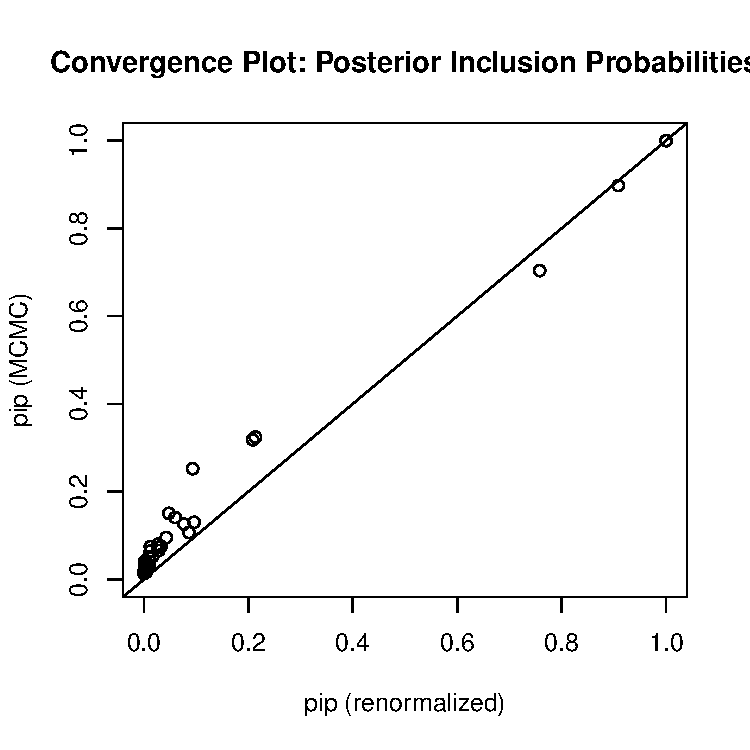
\includegraphics[width=.4\linewidth]{figure/diagnostics-1} 
\end{knitrout}

\end{frame}


\begin{frame}[fragile]\frametitle{Prediction}

\begin{knitrout}
\definecolor{shadecolor}{rgb}{0.969, 0.969, 0.969}\color{fgcolor}\begin{kframe}
\begin{alltt}
\hlstd{pred.bas} \hlkwb{=} \hlkwd{predict}\hlstd{(diabetes.bas,}
                   \hlkwc{newdata}\hlstd{=diabetes.test,}
                   \hlkwc{estimator}\hlstd{=}\hlstr{"BMA"}\hlstd{,}
                   \hlkwc{se}\hlstd{=}\hlnum{TRUE}\hlstd{)}
\hlkwd{mean}\hlstd{((pred.bas}\hlopt{$}\hlstd{fit}\hlopt{-} \hlstd{diabetes.test}\hlopt{$}\hlstd{y)}\hlopt{^}\hlnum{2}\hlstd{)}
\end{alltt}
\begin{verbatim}
## [1] 0.4552798
\end{verbatim}
\end{kframe}
\end{knitrout}

\end{frame}


\begin{frame}[fragile]\frametitle{95\% prediction intervals}
\begin{knitrout}
\definecolor{shadecolor}{rgb}{0.969, 0.969, 0.969}\color{fgcolor}\begin{kframe}
\begin{alltt}
\hlstd{ci.bas} \hlkwb{=} \hlkwd{confint}\hlstd{(pred.bas);} \hlkwd{plot}\hlstd{(ci.bas)}
\hlkwd{points}\hlstd{(diabetes.test}\hlopt{$}\hlstd{y,} \hlkwc{col}\hlstd{=}\hlnum{2}\hlstd{,} \hlkwc{pch}\hlstd{=}\hlnum{15}\hlstd{)}
\end{alltt}
\end{kframe}
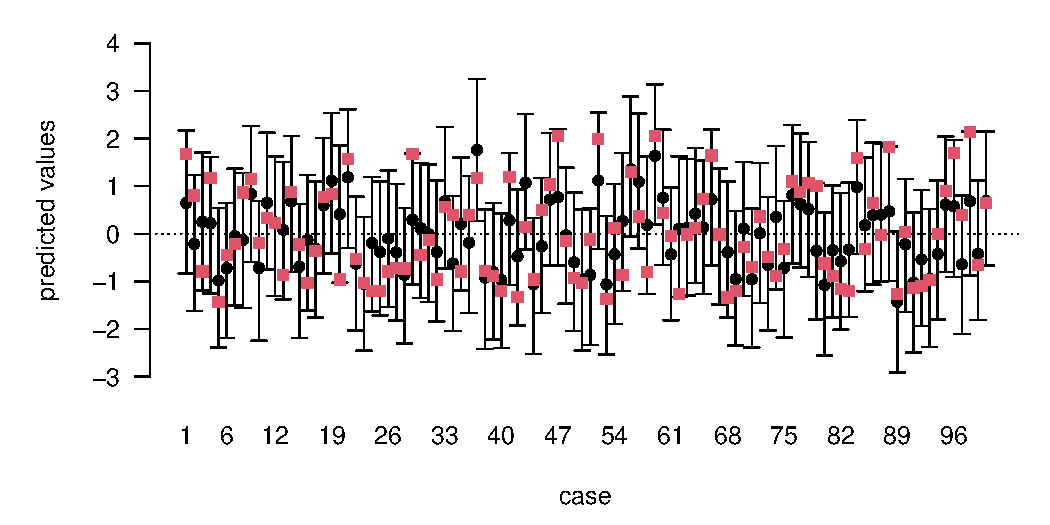
\includegraphics[width=\maxwidth]{figure/unnamed-chunk-6-1} 
\end{knitrout}



coverage is  $100$



\end{frame}

\begin{frame}\frametitle{Selection and Prediction}

\begin{itemize}
  \item  BMA  - optimal for squared error loss Bayes
  \item  HPM: Highest Posterior Probability model (not optimal for prediction) but for selection

\item MPM: Median Probabilty model (select model where PIP > 0.5)
 (optimal under certain conditions; nested models)

\item BPM: Best Probability Model - Model closest to BMA under loss
      (usually includes more predictors than HPM or MPM)
\end{itemize}

\end{frame}

\begin{frame}[fragile]\frametitle{Selection}
\begin{knitrout}
\definecolor{shadecolor}{rgb}{0.969, 0.969, 0.969}\color{fgcolor}\begin{kframe}
\begin{alltt}
\hlstd{pred.bas} \hlkwb{=} \hlkwd{predict}\hlstd{(diabetes.bas,}
                   \hlkwc{newdata}\hlstd{=diabetes.test,}
                   \hlkwc{estimator}\hlstd{=}\hlstr{"BPM"}\hlstd{,}
                   \hlkwc{se}\hlstd{=}\hlnum{TRUE}\hlstd{)}
\hlcom{#MSE}
\hlkwd{mean}\hlstd{((pred.bas}\hlopt{$}\hlstd{fit}\hlopt{-} \hlstd{diabetes.test}\hlopt{$}\hlstd{y)}\hlopt{^}\hlnum{2}\hlstd{)}
\end{alltt}
\begin{verbatim}
## [1] 0.4740667
\end{verbatim}
\begin{alltt}
\hlcom{#Coverage}
\hlstd{ci.bas} \hlkwb{=} \hlkwd{confint}\hlstd{(pred.bas)}
\hlkwd{mean}\hlstd{(diabetes.test}\hlopt{$}\hlstd{y} \hlopt{>} \hlstd{ci.bas[,}\hlnum{1}\hlstd{]} \hlopt{&}
     \hlstd{diabetes.test}\hlopt{$}\hlstd{y} \hlopt{<} \hlstd{ci.bas[,}\hlnum{2}\hlstd{])}
\end{alltt}
\begin{verbatim}
## [1] 0.98
\end{verbatim}
\end{kframe}
\end{knitrout}

\end{frame}


\begin{frame}\frametitle{Alternatives to MCMC}


\begin{itemize}
\item "Stochastic Search" (no guarantee samples represent posterior) \pause
\item Variational, EM, etc to find modal model \pause
\item in BMA all variables are included, but coefficients are
   shrunk to 0; alternative is to use shrinkage methods without point mass at zero \pause
  \item
  \item If $p > n$, can use a generalized inverse, but requires care for prior on $\g$!
\end{itemize}

\bigskip Model averaging versus Model Selection  -- what are objectives?


\end{frame}


\begin{frame}
  \frametitle{Effect Estimation}
  \begin{itemize}
  \item  Coefficients in each model are adjusted for other variables
    in the model
\item OLS:  leave out a predictor with a non-zero coefficient then
  estimates are biased!
\item Model Selection in the presence of high correlation, may leave
  out "redundant" variables;
\item improved MSE for prediction (Bias-variance tradeoff)

\item in BMA all variables are included, but coefficients are
   shrunk to 0
\item Care needed for "causal" questions   and confounder adjustment!    With confounding, should not use plain BMA.  Need to change prior to
  include potential confounders  (advanced topic)

  \end{itemize}


\end{frame}





\end{document}
